% ================================================================
%  前言 (Preface) 与 记号与术语 (Notation and terminology)
%  依据原书 PDF 第 vii--xix 页译出
% ================================================================

\chapter*{前言}
\addcontentsline{toc}{chapter}{前言}

\epigraph{一点小小的帮助，\\来自我的朋友们。}{}

\section*{定理之间的艺术}

新造型主义（Neoplasticism）——其最著名的代表是 Piet Mondrian——与\newterm{suprematism}{至上主义}{suprematism}——Kazimir Malévich 是其最纯粹的诠释者——是两种抽象绘画风格，它们常常出现在实变函数与\newterm{harmonic-analysis}{调和分析}{harmonic analysis}研究文献的图形与插图之中.

尽管彼此不同，这两种风格都主张简单形式的重要性，例如 Mondrian 笔下各边平行于画布坐标轴的矩形，或是 Malévich 笔下具有任意方向的矩形，并且都在构图中使用原色.

一个典型的例子是 Calderón--Zygmund 算法. 给定定义在平面矩形 $R$ 上的非负可积函数 $f$，以及一个严格大于其平均值的固定数 $m$，即 $m > f_R = \frac{1}{\mu(R)} \int_R f$，我们把 $R$ 二进地分成四个矩形，并保留其中 $f$ 的平均值大于 $m$ 的那些. 接着，我们把其余的矩形同样进行二进细分，并沿用同样的准则，保留那些相应平均值大于 $m$ 的矩形，如此继续下去. 在过程结束时，我们将得到包含于原来 $R$ 的一列矩形 $R_j$，它们满足性质 $m < f_{R_j} \le 4m$；并且由 Lebesgue 微分定理，在它们的并集之外几乎处处有 $f(x) \le m$.

如果我们把属于同一代（即边长相同）的序列成员涂上相同的颜色（红、蓝、黄、黑，……），结果看上去就会像一幅 Mondrian 的画. 而由参数 $m$ 的不同值得到的一系列 ``Mondrian 画'' 将为我们提供关于作用在函数 $f$ 上的奇异积分算子之性状的关键信息.

\begin{center}
  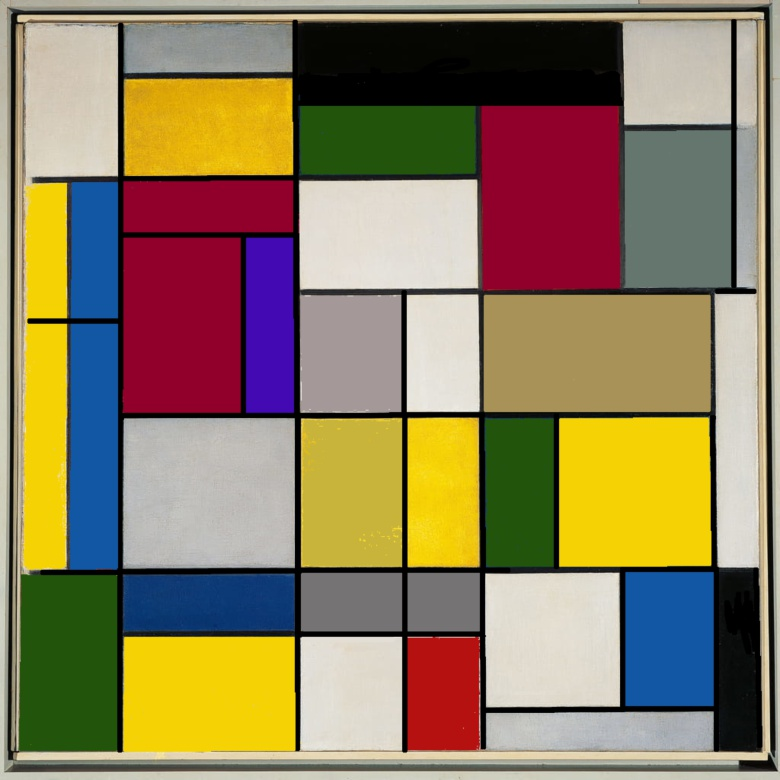
\includegraphics[width=0.55\textwidth]{figs/preface-mondrian.jpeg}

  \smallskip
  {\small\itshape Piet Mondrian 风格的新造型主义绘画.}
\end{center}

\smallskip
然而，调和分析中还有另一些重要的算子，它们涉及欧氏空间中许多方向上的希尔伯特变换，对它们的理解要求按这些不同方向作矩形分解（第 5 章考虑的所谓圆盘乘子便是一个好例子）. 在这些情形中，所得的图像会更像 Malévich 至上主义的构图.

\begin{center}
  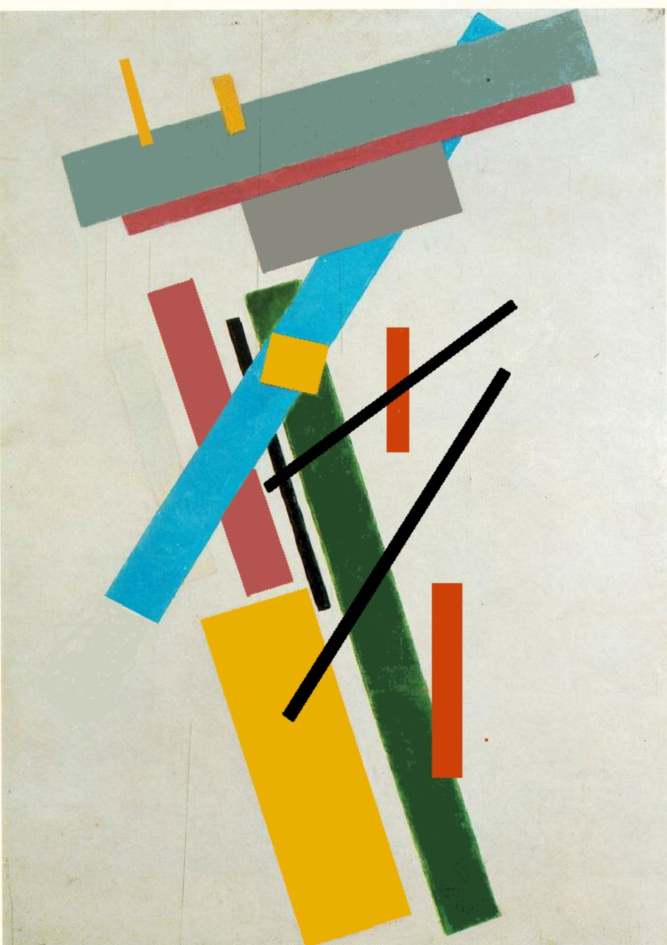
\includegraphics[width=0.4\textwidth]{figs/preface-malevich.jpeg}

  \smallskip
  {\small\itshape 效法 Kazimir Malévich 至上主义的构图.}
\end{center}

\smallskip
我希望这些幼稚的离题之谈有助于为本书的书名辩护——至少是为书名的前半部分，因为后半部分（第 5 至 9 章）并不那么容易纳入这样的比喻；在那里，振荡积分（驻相、Fresnel 衍射、高斯和、van der Corput 估计、Cornu 螺线等）的盛行会让人联想到别样的绘画风格. 大胆一点说，可以把它们与 Vincent van Gogh 的名作《星月夜》联系起来，正如 2009 年 6 月在马德里召开的一次分析学会议的海报所做的那样: 在那幅画中融入了第 5 章二维 Bochner--Riesz 猜想证明中的若干至上主义元素.

\begin{center}
  
\includegraphics[width=0.62\textwidth]{figs/preface-starrynight.jpeg}

  \smallskip
  {\small\itshape Fernando Chamizo 在 Van Gogh《星月夜》上的至上主义介入.}
\end{center}

\section*{本书的核心}

第 1 章可以看作一首嬉游曲. 让我们把\termcn{数学俳句}定义为这样的陈述: 其表述不需要复杂的术语，其证明锋利而简短，只要掌握了恰当的视角，无须花费太大力气便能理解. 所选的这些俳句中有一些在后续章节中有应用，例如关于凸集的 Fritz John 引理（它使我们可以把由凸集构成的基之微分性质的分析化归为平行多面体的情形），但另一些的入选仅仅是因为我喜欢它们.

第 2 章的背景是经典的 Vitali 覆盖引理，它对欧氏空间中的方体或球成立，而对其他微分基一般不成立；同时还有集族覆盖性质与相应极大算子弱型估计之间的关系. 一个标准的线性化把非线性极大函数的有界性化归为一族线性算子的一致有界性，取它们的伴随（对偶）算子，我们就能用这些伴随所蕴含的覆盖性质来读出弱型不等式.

本章还处理指数型覆盖（它为各边平行于坐标轴的平行多面体所满足），以及 Antoni Zygmund 关于三维欧氏空间中的单调平行多面体族的一个猜想的肯定回答. 本章还有针对带缺项方向的平行多面体所对应极大函数的至上主义式处理.

第 3 章主要讨论 Kakeya 集或 Besicovitch 集的理论，即测度为零、在空间每个方向上都包含一条单位直线段的紧集. 考虑 $\R^n$ 中由离心率（高/半径，或高/底方体边长）等于 $1/\delta$ 的柱体（或平行多面体）构成的族 $\mathcal{B}_\delta$，$0 < \delta < 1$. 给定局部可积函数 $f$，定义
\begin{align*}
  M_\delta f(x) = \sup_{x \in R \in \mathcal{B}_\delta} \frac{1}{\mu(R)} \int_R |f(y)| \, \mathrm{d}\mu(y).
\end{align*}
关于这个极大函数有一个猜想:

\begin{conjecture*}
对每个 $n \ge 2$，存在常数 $C(n)$ 与 $a(n)$，使得对每个 $\delta > 0$，下列估计成立:
\begin{align*}
  \|M_\delta f\|_n \le C(n) \, [1 + |\log \delta|]^{a(n)} \, \|f\|_n.
\end{align*}
\end{conjecture*}

下面是第 3 章的主要结果.

\begin{theorem*}[Kakeya 极大函数定理]
上述猜想在维数 $n=2$ 时成立.
\end{theorem*}

这个定理的一个直接推论是: 二维的每个 Kakeya 集必有等于 $2$ 的 Minkowski 维数（计盒维数），再加一些额外的论证，它也蕴含对 Hausdorff 维数同样的结论. 它的证明可追溯到 1972 年，其概要版 \cite{b41} 于 1975 年刊于 Bulletin of the AMS. C.~Fefferman 在 1974 年温哥华国际数学家大会上题为 ``Recent progress in classical Fourier analysis'' 的大会报告中引用了它. 含有详细证明的论文在同一年（1974 年）被 American Journal of Mathematics 接受，但因积压过多，迟至 1977 年才刊出，见 \cite{b65}. 近来若干作者撰写了关于 Kakeya 集的结果年表，把这一定理的日期记为 1977 年；而严格地说，它在早五年时便已获得，并于 1974 年宣布. 它是我在芝加哥大学博士论文的一部分. 很自然地，我被鼓励去尝试高维的情形，但结果表明这是一项非常艰巨的任务，时至今日仍是一个富有挑战性的公开问题.

尽管如此，有一点是清楚的: 它的解决将由一个恰当的高维覆盖引理所蕴含，而为此自然可以先得到若干特殊情形，它们在如今的文献中以``丛''（bush）与``刷''（brush）构型这样形象的名字著称，即所涉及的柱体（或平行多面体）共享一个公共点（丛），或都与其中某个给定者相交（刷）. 对于这两种构型（丛或刷），都有简单的几何论证给出重叠函数的正确估计，但在当时（1974 年），这些观察被认为不够格单独发表. 多年之后，Jean Bourgain 与 Tom Wolff 重新发现了这些粗针特殊构型的性质，并利用它们得到了维数大于 $2$ 的 Kakeya 集分形维数的下界.

雄心一点，我们可以把下述``至上主义覆盖引理''表述为一个猜想:

\begin{definition*}
平行多面体的有限族 $\{R_i\}$ 具有\termcn{稀疏性}（P），若对每个 $j$,
\begin{align*}
  \mu\Big( R_j \setminus \bigcup_{k \ne j} R_k \Big) \le c \, \mu(R_j),
\end{align*}
其中 $c < 1$ 是一个固定的正常数.
\end{definition*}

\begin{definition*}
平行多面体的有限族 $\{R_\alpha\}$ 称为一个\termcn{丛}（bush），如果它们有非空的交，且该族满足性质（P）.
\end{definition*}

\begin{conjecture*}[至上主义覆盖引理]
给定 $\R^n$ 中平行多面体的族 $\mathcal{B}$，有
\begin{align*}
  \sup_{\substack{\{R_j\} \subset \mathcal{B} \text{ 满足\,(P)} }}
  \frac{1}{\mu(\bigcup_j R_j)} \Big\| \sum_j R_j \Big\|_p
  \;\le\; C_p
  \sup_{\substack{\{R_\alpha\} \subset \mathcal{B} \text{ 是丛} }}
  \frac{1}{\mu(\bigcup_\alpha R_\alpha)} \Big\| \sum_\alpha R_\alpha \Big\|_p,
\end{align*}
这里我们滥用记号，用 $R = R(x)$ 表示集合 $R$ 的示性函数.
\end{conjecture*}

第 4 章讨论傅里叶变换的乘子，着重强调奇异积分加权不等式的角色，循着 Benjamin Muckenhoup \cite{b94} 以及 Ronald Coifman 与 Charles Fefferman \cite{b82} 的开创性工作. 1974 年初，在与 C.~Fefferman 合作、1976 年发表的一项工作（见 \cite{b84}）中，人们观察到: 给定 $\R^n$ 中任意局部可积函数 $f$ 与实数 $r > 1$，则 $M(f^r(x))^{1/r}$——其中 $M$ 表示 Hardy--Littlewood 极大函数——是一个 $A_1$ 类中的权重，且界与函数 $f$ 无关. 这一观察对第 5 章二维 Bochner--Riesz 算子猜想的至上主义式证明是至关重要的，它使那些算子可以用 Kakeya 极大函数来估计. 我为这一方法之美所折服，常在我的报告里断言: 直接的 $L^p$ 不等式并非问题的要害，更好的策略是去寻找带适当权重的 $L^2$ 估计.

在 1976--77 学年，Eli Stein 请我在普林斯顿大学讲授他的调和分析研究生课程，内容是当时关于奇异积分加权不等式的最新结果. 对我而言，这是整理这部分材料的好机会，也极具挑战性，因为 Carl Herz、Alex Nagel、Alice Chang 与 José Luis Rubio de Francia 那一年正在普林斯顿数学系访问，并出席了我的讲课. 那些讲义的笔记后来又用于 1978 年夏在 El Escorial 举行的调和分析会议上所授的短课，并收入其会议录. 我相信它们影响了后来 García-Cuerva 与 Rubio de Francia \cite{b4} 以及 Stein \cite{b13} 对这一主题的表述. 第 4 章可以视为它们的一个更新版本.

第 5 章从 C.~Fefferman 对圆盘乘子猜想的反例开始，其中用到了 Kakeya 集的性质，这一反例正是本书所强调的研究进路的源头. 接着是二维 Bochner--Riesz 算子的有界性；对这一结果，文献中另有两种证明，分别由 Lennart Carleson 与 Per Sjölin \cite{b103} 以及 Lars Hörmander \cite{b117} 给出，但其所用方法不同于这里采用的至上主义观点.

与 Kakeya 极大定理一起，我们的证明还涉及若干平方函数估计. 其中一些已知在一般维数成立: 设 $\mathcal{L} = \{R_\nu\}$ 是 $\R^n$ 中内部两两不交的全等平行多面体构成的格，考虑由公式 $\widehat{P_\nu f}(\xi) = R_\nu(\xi) \widehat{f}(\xi)$ 定义的傅里叶乘子 $P_\nu$. 定义平方函数 $G(f) = \big( \sum_\nu |P_\nu(f)|^2 \big)^{1/2}$. 则下列不等式成立:
\begin{align*}
  \int_{\R^n} |Gf(x)|^2 \, w(x) \, \mathrm{d}x \ \lesssim_r \
  \int_{\R^n} |f(x)|^2 \, [M_s w^r(x)]^{1/r} \, \mathrm{d}x,
\end{align*}
其中 $r > 1$，$M_s$ 表示强极大函数，而 $f$ 与 $w > 0$ 是任意的函数: $f$ 属于 Schwartz 类，$w$ 局部可积.

但还有另一些平方函数，其确切的有界性只在二维已知. 给定 $\delta < 1$，定义一个 $\delta$-板（plate）为高 $\delta$、半径 $\delta^{1/2}$ 的柱体. 设 $\{B_j\}$ 是与单位球面相切的两两不交的 $\delta$-板族，且对每个 $j$，$f_j$ 是傅里叶变换支于 $B_j$ 的光滑函数.

\begin{conjecture*}[至上主义平方函数引理]
成立估计
\begin{align*}
  \Big\| \sum_j f_j \Big\|_{2n/(n-1)} \ \lesssim \
  \Big\| \Big( \sum_j |f_j|^2 \Big)^{1/2} \Big\|_{2n/(n-1)},
\end{align*}
其中的常数与 $\delta$ 无关.
\end{conjecture*}
当 $n = 2$ 时指数 $2n/(n-1)$ 恰为 $4$，这对该猜想的二维证明大有助益；而在高维，它仍然是公开的.

可以说，二维的理论如今已被充分理解，本章试图对其主要面貌作一个相当完整的陈述，包括傅里叶变换在圆周上的限制、角平方函数的估计、Bochner--Riesz 平均的几乎处处收敛，以及沿平面曲线的希尔伯特变换的 $L^p$ 估计.

第 6 章是对第 5 章的补充，对关于球乘子的那个被否证的猜想给出了一个肯定的回答: 若把 $L^p(\R^n)$（$\frac{2n}{n+1} < p < \frac{2n}{n-1}$）换成 $L^p_{\mathrm{rad}} L^2_{\mathrm{ang}}(\R^n)$，则猜想成立，球乘子算子在这一档混合范数空间上有界. 在角向部分取 $L^2$ 范数有助于击败 Kakeya 集这个对手，从而建立起一个定理. 证明的方法如今有所不同，依赖于任意阶贝塞尔函数的十分精确的渐近公式. 这一研究进路受到信号理论中带限函数研究的影响，特别是长球面波函数级数的收敛性，以及 Dirichlet 边界条件下单位球上拉普拉斯算子本征函数级数的展开理论.

第 7 章讨论泊松求和公式，它可以用一个格 $\mathcal{L}$ 及其对偶格 $\mathcal{L}^*$ 来表述: 由置于 $\mathcal{L}$ 的顶点处的 $\delta$ 函数之和给出的缓增分布，其傅里叶变换等于支在 $\mathcal{L}^*$ 顶点处的 $\delta$ 函数之和（至多差一个由基本胞腔体积决定的因子）.

除了众多重要的数学应用之外，该公式在晶体学中也很要紧，因为在那里，分子的电子密度函数的傅里叶变换通常与其 X 射线谱相联系，历史上，这一观察曾是理解固体的关键一步. 晶体学范式说: 周期结构产生锐利的 Bragg 峰，而这些峰的分布的知识应能允许我们重建晶体（也许要除去丢失的相位，但那是另一个问题）. X 射线晶体学家们编制出了晶体的目录及其对称群的分类. 但是这座大厦在上世纪八十年代中期遭受了一次地震般的冲击: 准晶体被发现了——那是一些材料，其 X 射线谱呈现清晰的 Bragg 峰，却带有理论所不允许的五重对称性.

1986 年我在苏黎世联邦理工学院（ETH）访问，参加了由 John Garnett 组织的调和分析学期活动，其间我听了好几场关于这一问题的报告. 我的第一反应是追问是否还有别的泊松公式，经过几周的工作，我得到了答案: 没有别的公式了. 更精确地说: 给定两个离散点集 $X = \{x_j\}$ 与 $Y = \{y_k\}$，若缓增分布 $\sum \delta_{x_j}$ 的傅里叶变换等于 $\sum \delta_{y_k}$，则 $X$ 与 $Y$ 必是基本胞腔体积为 $1$ 的互相对偶的格. 这就是第 7 章的开篇定理，它发表 \cite{b154} 于法国科学院的 Comptes Rendus——在此之前，我的几位朋友，全是杰出的调和分析学家，都敦促我发表，因为据他们相告，这个证明对他们而言是新的. 若在早些年，它本可以被视为晶体学的一条基本定理，但准晶体的出现改变了晶体的经典定义，给数学家留下了如下任务: 为理解新材料的 X 射线谱，去研究并分类更一般的泊松求和公式. 依我之见，这项任务还远未完成.

在前几章考虑过 $\R^k$ 中球的傅里叶变换之后，对泊松求和公式的讨论不可避免地把我们引向数论中的格点问题，即估计以原点为中心、$r$ 为半径的球内格点数时，用球的体积去近似所造成的误差项. 沿 Hardy 的路线，泊松公式使我们能把误差项写成含贝塞尔函数与算术函数 $r_k(m)$ 的解析表达式，其中 $r_k(m)$ 计数把 $m$ 表为 $k$ 个平方和的表法数. 这里无意对如此重要而有趣的理论作公允的综述，只想强调泊松公式在为误差项产生解析可处理的表达式方面的作用. 引 Fernando Chamizo 的话: ``泊松公式容许我们把数格点换成数波''. 与前面各章的 Bochner--Riesz 问题相比，一个显著的差别是: 这里的困难在于二维和三维，而对 $k \ge 4$，由于 $r_k(m)$ 的行为更规则，误差项的确切估计是已知的.

本章还包含把理论推广到平面上凸区域的工作，其精神源自 Feynman 的路径积分，它有助于理解并界定在重要情形 $k=2$ 中关于该误差项的 Hardy 猜想的困难所在. 本章还有若干关于 X 射线谱学中相位恢复问题的杂评，它们与高斯和有关.

调和分析与数论的交界面如此广阔、成果如此丰富，以至于第 8 章只能指望指出其中若干论题——也许不是最重要的，但我希望多少是有意义的. 在那个领域里，Riemann 与 Hardy 的名字无处不在；``圆法''、``Vinogradov 均值定理''或``三角和的 Weyl 估计''等技巧举足轻重；而前面提到过的格点计数、Waring 问题或 Goldbach 猜想等问题，则一直是两个学科之间十分有趣的数学互动的源泉.

为给第 8 章定位，一个合适的起点是 Zygmund 书中研究特殊三角级数的部分. 在那里我们可以找到缺项级数的性质，即形如 $\sum_k a_k \exp(2\pi i n_k x)$、频率几何式增长的级数: $n_{k+1}/n_k > \rho > 1$. 书中证明: 若这样的级数是某个可积函数的\newterm{fourier-series}{傅里叶级数}{Fourier series}，则该函数的任何正幂次也必可积，且相应的 $L^p$ 范数都与其 $L^2$ 范数等价. 如今我们还可以把上述论断精确化: 该级数还属于空间 BMO（有界平均振荡）. Zygmund 这部论著的细心读者会在那一部分发觉缺少了频率按 $k$ 次幂增长时的相应命题. 初步的考虑给出限制 $p < 2k$: 若可积函数的傅里叶级数的频率都是 $k$ 次幂，则该函数必属于 $L^p$. 但 $p < 2k$ 时的这一断言仍是一个突出的困难公开问题，即使在 $k = 2$ 的情形——那里我们对高斯和有非常精确的信息. 当我们把问题用傅里叶级数的乘子算子来重述时，会发现相应的核与第 4 章考虑的奇异积分大不相同. 这里恰可想起 Henryk Iwaniec 的评论: ``在调和分析里，我们是把好核作用于复杂的函数；而在数论里，我们是把难的核作用于非常光滑的函数.''

在本章中，读者会看到关于这一问题的一些观察和特殊情形，但没有它的解. 不过，未能补全 Zygmund 之书的沮丧，可以因如下的发现得到缓解: 三角级数
\begin{align*}
  \sum_{n \ge 1} n^{-(1+\delta)} e^{2\pi i n^k \cdot x}
\end{align*}
的图象的 Minkowski 维数是可以精确计算的，而这些级数在 Riemann 的学位论文 \cite{b194} 中已被考虑过，在那里他还推广了当时通行的积分与导数的概念，除此之外还有别的有趣论题.

本章以数论对傅里叶级数的一种收敛方法的应用作结，其中的部分和如今是按系数的大小来选取的. 由于前一章描述的理由，这是在晶体学中很自然的一种方法.

第 9 章从对原子 Born--Oppenheimer 理论的简快介绍开始，包括对原子序数为 $Z$ 的中性原子的基态的 Thomas--Fermi 与 Hartree--Fock 近似的一种印象派式描述. 其目的在于说明三角和的 Weyl 估计在原子能量振荡中所起的作用，这一现象对从量子力学第一性原理出发理解化学元素周期表具有意义. 这是 C.~Fefferman 与 Luis Seco \cite{b206} 在对大原子基态能量渐近公式的 Dirac--Schwinger 修正作严格处理时发现的一个效应，随后在若干出版物中又被深入分析 \cite{b200,b201,b207,b209,b223}. 本章只打算为认真关心该理论的读者提示进一步的读物，且在某种意义上，它是第 1 章数学俳句思想的对应物. 但它足以传达调和分析的深度与多样性: 从欧氏空间中平行多面体的初等几何开始，到关于原子能量振荡的量子力学问题结束.

幸运的是，经典傅里叶分析有若干杰出的论著，例如 Zygmund 的 \emph{Trigonometric series} \cite{b17}，Stein 的 \emph{Singular integrals and differentiability properties of functions} \cite{b12}，以及 Stein 与 Guido Weiss 的 \emph{Introduction to Fourier analysis on Euclidean spaces} \cite{b14}；我假定读者对它们的内容已有所知. 本书的主要目的是呈现若干超出这些著名专著范围的结果——这一抱负听上去比实际上更为雄心勃勃. 一份更详尽的有益参考文献清单见文末参考文献的开头部分.

\section*{几则个人感言}

有一次，我参加一个报告，报告人在黑板上写下``分析学家 = 猎人''这句话，并如此解释: ``分析学家像猎人一样，把大部分时间花在总部里打磨他的工具. 他有时出去打猎，但很快就回到家中，继续磨快他的刀.''

年龄不是一个特别有趣的话题，但它通常有助于获得某种视角. 上世纪七十年代初，作为芝加哥大学的研究生，我有幸亲眼见证了 Alberto Calderón 与 Antoni Zygmund 学派发展起来的奇异积分理论对线性偏微分方程的成功冲击，它解决并照亮了诸如双曲方程 Cauchy 问题的唯一性、椭圆边值问题、局部可解性的刻画或指标定理等基本问题. 在导师的指点下，我熟读了原始文献，即 Calderón--Zygmund、Kohn--Nirenberg、Beals--Fefferman、Atiyah--Singer 以及其他许多人的著作，这促使我在七十年代末在马德里康普鲁滕塞大学开设了一门研究生课程，其讲义以 \emph{Pseudodifferential operators and applications}（伪微分算子及其应用）为题在当地出版. 在那些年里，发展伪微分算子与傅里叶积分算子的理论，并猎取它们对线性偏微分方程的应用，是傅里叶分析主流的活动. 这场活动也催生了一批综述与专著，并在 Lars Hörmander 那部里程碑式的巨著 \cite{b8} 中达到顶点——我认为它把这一主题封闭了几十年.

主流随后改变了方向，转而注意非线性问题. 五十年代末 E.~de Giorgi 与 J.~Nash 的开创性工作如同一块罗塞塔石碑，使人们得以理解椭圆与抛物型的非线性方程——例如极小曲面所满足的方程——并为处理自由边界问题与相变开辟了道路；在那里，奇异积分理论再次极为有用. 还有 J.~Leray 以及其他许多人对流体力学方程的贡献；在那里，傅里叶分析学家磨快的工具再一次成为关键.

粗略地说，我们可以把这些视为那些年里调和分析学家的主要猎场. 不过也有其他重要的活动领域，例如 J.~von Neumann 与 H.~Weyl 对量子力学的严格数学奠基，或者 Hardy--Littlewood--Ramanujan 对数论的杰出贡献. 但在那里，尤其是在数论中，正如 H.~Iwaniec 指出的，所需估计中涉及的核的性质偏离了 Calderón--Zygmund 范式.

我与多位杰出的合作者一起，在那些主流领域工作并发表过文章. 但我也关心过另一些较为``旁系''的问题，例如前面提到的 Zygmund 关于积分微分的猜想、Kakeya 集与 Bochner--Riesz 求和、推广的泊松求和公式，以及 Riemann 图象的分形维数. 本书主要就是关于这些旁系主题的，它源自 2020 年冬季学期我在穆尔西亚大学讲授的一门研究生课程. 新冠疫情使这门课在随后几年未能继续，但尽管我至今仍不很明白完成这些讲义的理由，我还是力图把我多年的想法有条理地呈现出来，或许带着一点夸张的自负: 某些读者也许能从中找到未来研究的灵感.

\section*{致谢}

我怀着极大的愉快向所有尊敬的研究合作者致谢，他们的贡献丰富了本书的内容. 我要特别感谢 Pablo Fernández Gallardo 与 Fernando Chamizo，他们宝贵的洞见与建议对提升本书的表述质量与协调各章内容起到了关键作用.

我还要对穆尔西亚大学表示感谢，奠定本书基础的研究生课程正是在那里讲授的；同时感谢数学科学研究所（ICMAT）的 Severo Ochoa 项目慷慨的经费资助.

最后，我感激 Alfonso Núñez 与 Irene Quintero 出色的专业技艺，他们把我最初的手写稿转化为规范的 LaTeX 格式，使之得以面向更广的读者.

\begin{flushright}
  马德里，2024 年 8 月

  \medskip
  Antonio Córdoba
\end{flushright}

\vspace{1cm}

% ================================================================
%                        记号与术语
% ================================================================

\chapter*{记号与术语}
\addcontentsline{toc}{chapter}{记号与术语}

\begin{itemize}
\item
  $\chi_A$ 是集合 $A$ 的示性函数的标准记号. 为了简化记号，在不致混淆时，将简写为 $A(x) = \chi_A(x)$:
  \begin{align*}
    A(x) = \chi_A(x) =
    \begin{cases}
      1, & \text{若 } x \in A, \\
      0, & \text{若 } x \notin A.
    \end{cases}
  \end{align*}

\item
  给定定义在区域 $D$ 上的两个实函数 $f$ 与 $g$，记号 $f \lesssim g$ 表示存在有限正常数 $C$，使得对每个 $x \in D$ 都有 $f(x) \le C g(x)$. 类似地，$f \gtrsim g$ 表示对 $x \in D$ 有 $f(x) \ge C g(x)$. 而 $f \simeq g$ 表示 $f \lesssim g$ 且 $g \gtrsim f$.

  记号 $\ll$、$\gg$ 分别等同于 $\lesssim$ 与 $\gtrsim$. 它们由 I.~Vinogradov 引入，主要用于数论文献；而 $\lesssim$、$\gtrsim$ 与 $\simeq$ 是调和分析中的常用记号.

\item
  $[x]$ 表示 $x$ 的整数部分；$\{x\}$ 表示 $x$ 的小数部分.

\item
  $J_k$ 表示 $k$ 阶第一类贝塞尔函数.

\item
  除非另有明文说明，$\mu(A)$ 表示集合 $A \subset \R^n$ 的\newterm{lebesgue-measure}{Lebesgue 测度}{Lebesgue measure}. 在某些场合也使用记号 $|A| = \mu(A)$.

\item
  我们用 $\fint_R f$ 表示平均值:
  \begin{align*}
    \fint_R f = \frac{1}{\mu(R)} \int_R f(x) \, \mathrm{d}\mu(x).
  \end{align*}

\item
  \newterm{fourier-transform}{傅里叶变换}{Fourier transform}:
  \begin{align*}
    \widehat{f}(\xi) = \int_{\R^n} e^{-2\pi i x \cdot \xi} \, f(x) \, \mathrm{d}x.
  \end{align*}

\item
  Mellin 变换:
  \begin{align*}
    M f(s) = \int_0^\infty t^{-is} f(t) \, \frac{\mathrm{d}t}{t}.
  \end{align*}

\item
  \newterm{convolution}{卷积}{convolution}:
  \begin{align*}
    f * g(x) = \int_{\R^n} f(x - y) \, g(y) \, \mathrm{d}y.
  \end{align*}
  记号 $f *_i g$ 表示仅在第 $i$ 个变量上作卷积.

\item
  $M(f)$ 表示 Hardy--Littlewood 极大函数.

\item
  $M_s(f)$ 表示强极大函数.

\item
  $M_N(f)$ 表示 Kakeya 极大函数（离心率为 $N$ 的矩形）.

\item
  主值积分:
  \begin{align*}
    \mathrm{p.v.} \int_{\R^n} g(x) \, \mathrm{d}x
    = \lim_{\varepsilon \to 0^+} \int_{|x| \ge \varepsilon} g(x) \, \mathrm{d}x.
  \end{align*}

\item
  沿方向 $v$ 的希尔伯特变换:
  \begin{align*}
    H_v f(x) = \lim_{\varepsilon \to 0^+} \int_{|t| \ge \varepsilon} \frac{f(x - vt)}{t} \, \mathrm{d}t.
  \end{align*}

\item
  $\mathrm{d}\sigma(\bar{y})$ 是 $\R^n$ 中单位球面 $S^{n-1}$ 上的 Lebesgue 测度.

\item
  $L^p_{\mathrm{rad}} L^2_{\mathrm{ang}}(\R^n)$ 是满足
  \begin{align*}
    \Big[ \int_0^\infty \Big( \int_{S^{n-1}} |f(r\bar{y})|^2 \, \mathrm{d}\sigma(\bar{y}) \Big)^{p/2} r^{n-1} \, \mathrm{d}r \Big]^{1/p} < \infty
  \end{align*}
  的函数 $f$ 所构成的空间.
\end{itemize}
